\documentclass[dvipsnames] {beamer}
\usepackage{cmlgc}
\usepackage{comment}
\usepackage{tikz}
\usefonttheme{serif}     % Font theme: serif
\usepackage[T2A]{fontenc}
\usepackage[utf8]{inputenc}
\usepackage[english]{babel}
\usepackage{amssymb,amsfonts,amsmath,mathtext,cite,enumerate,float} %подключаем нужные пакеты расширений
% \usepackage{cyrillic}
\usepackage{color, colortbl}
\usepackage{multirow}
\usepackage{graphicx}
\usepackage{graphics}
\usepackage{multirow}
\usepackage{url}
\usepackage{hyperref}
\usepackage{animate}
\usepackage{pifont}
\usepackage{wasysym}
\usepackage{marvosym}
\usepackage{appendixnumberbeamer} 
\usepackage{pgfpages}
\usepackage{systeme,mathtools}
\usepackage{mathtools}
\usepackage{listings}
\usepackage{xcolor} % for setting colors
\usepackage{mhchem}


\usepackage{ragged2e} %выравнивание текста по ширине слайда (\justifying)
%\setbeamercolor{background canvas}{bg=violet}

\usetheme{Madrid}
%\usecolortheme{crane}

%=================================================

\defbeamertemplate*{footline}{mytheme}{%
  \leavevmode%
  \hbox{%
    \begin{beamercolorbox}[wd=.2\paperwidth,ht=3ex,dp=1ex,center]{author in head/foot}%
      \usebeamerfont{author in head/foot}\insertshortauthor
    \end{beamercolorbox}%
    \begin{beamercolorbox}[wd=.7\paperwidth,ht=3ex,dp=1ex,center]{title in head/foot}%
      \usebeamerfont{title in head/foot}\insertshorttitle
    \end{beamercolorbox}%
    \begin{beamercolorbox}[wd=.1\paperwidth,ht=3ex,dp=1ex,right]{date in head/foot}%
      %\usebeamerfont{date in head/foot}\insertshortdate{}\hspace*{2em}
      %\insertframenumber{} / \inserttotalframenumber\hspace*{2ex} %номер текущего слайда / общее число слайдов
      \insertframenumber{} \hspace*{5ex}  %номер текущего слайда
  \end{beamercolorbox}}%
  \vskip0pt%
}
\usebeamertemplate{mytheme}
\beamertemplatenavigationsymbolsempty

\defbeamertemplate*{frametitle}{boldTitle}{%
  \begin{beamercolorbox}[wd=\paperwidth,ht=3ex,dp=3pt,center]{title in head/foot}%
    %        \ \textit{\textbf{\insertframetitle}} % курсивный заголовок слайда 
    \ \textbf{\insertframetitle}
  \end{beamercolorbox}
}
\usebeamertemplate{boldTitle}
\setbeamercovered{dynamic}

\setbeameroption{hide notes} % Only slides
%\setbeameroption{show only notes} % Only notes
%\setbeameroption{show notes on second screen=right} % Both
%\setbeamertemplate{note page}[plain]


%=================================================
% \titlegraphic{\includegraphics[width=\textwidth]{logo_conf.png}}

\addtobeamertemplate{title page}{\centering \includegraphics[scale=0.265]{jinr_nica_logo_1.png}}{}
\addtobeamertemplate{title page}{\centering \includegraphics[scale=0.25]{dubna_town.pdf}}{}
%\addtobeamertemplate{title page}{\centering \includegraphics[scale=.05]{vblhep_logo.png}}{} 
%\addtobeamertemplate{title page}{\centering \includegraphics[scale=0.095]{wpcf2018_2.png}}{}
\vskip -1cm
\title[\bf Russia, Dubna, XIV Workshop on Particle Correlations and Femtoscopy]
      {\textbf{\large {Femtoscopy with identified particles for NICA/MPD}}}

      \author[\bf P.~Batyuk]{\textit{\textbf{{\footnotesize \underline{P.~Batyuk}, L. Malinina, K. Mikhaylov, G.Nigmatkulov}}}} 
      %on behalf of the MPD collaboration} 
      \institute{\bf Dubna, Joint Institute for Nuclear Research}

      \date{{\textbf{June 4, 2019}}}  
      % \newpage \footnotesize April 14, 2016}}

      \lstset{
        %    frame=tb, % draw a frame at the top and bottom of the code block
        tabsize=4, % tab space width
        showstringspaces=false, % don't mark spaces in strings
        %   numbers=left, % display line numbers on the left
        commentstyle=\color{blue}, % comment color
        keywordstyle=\color{blue}, % keyword color
        stringstyle=\color{red} % string color
      }

      \begin{document}
      \maketitle
      \note{Hello, \\
        First of all, many thanks to organizers for a given possibility to do a talk within the Workshop.
        It is a great pleasure for me to present results of investigations of our Physics Working Group within the MPD experiment on Femtoscopy with identified
        particles. Participants contributed essentially to this work are listed in the slide.}

      \begin{frame}
        \frametitle{\bf \centering Outline:}
        \bf
        \begin{itemize}
        \item Motivation
        \item Hybrid vHLLE+UrQMD model 
        \item Comparison with BES-I STAR
          \begin{itemize}
          \item pions
          \item first results with kaons {\color{red} (NEW!)}
          \end{itemize}
        \item Package for Femtoscopic Analysis
        \item Summary
        \end{itemize}
        \note{\footnotesize In the slide I am presenting a short outline what I am planning to speak about.
          In the beginning, a few slides describing motivation of our research
          are given. Since, at the moment, our activity is concentrated on model studies, I plan to present a Monte-Carlo generator used for the work pointing out its
          features for our studies. The second step we did is related to a comparison of model output with existing experimental data, of course, in sense of
          femtoscopy observables we extracted from the model. As a reference point we took into account STAR pion data to do the comparison. A new point here is
          our new calculations done for charged kaons, where we obtained preliminary results on femtoscopic observables I am planning to discuss.
          In the report I also should stress out attempts to go to analysis of, I would say, real reconstructed output from MPD. To achieve this point,
          we have to develop an appropriate software taking into account realistic effects for different subdetector systems of the experiment.
          A package to be presented in the talk is considered as a candidate for such a software.}
      \end{frame}

      \begin{frame}[shrink=40]
        \bf
        \vskip -.4cm
        \frametitle{\bf \centering Femtoscopy formalism}
        \begin{columns}[c]
          \column{.30\textwidth}
          \begin{block}{}
            \begin{figure}[H]
              \includegraphics[width=1.\linewidth]{corr_femto1.png}
            \end{figure}
          \end{block}
          \column{.65\textwidth}
          \begin{block}{{\bf \centering Correlation femtoscopy:}}
            %     {\tiny
            Measurement of space-time characteristics $R$, $c_{\tau}$ of particle production
            using particle correlations due to the effects of quantum statistics (QS) and final state interactions (FSI)
            %      }
          \end{block}
          \begin{block}{{\bf \centering Two-particle correlation function:}}
            %      \tiny{
            \begin{center}
              {\bf theory:     $C(q) = \dfrac{N_{2}(p_{1}, p_{2})}{N_{1}(p_{1}) N_{2}(p_{2})}, C(\infty) = 1$
                
                experiment: $C(q) = \dfrac{S(q)}{B(q)}, q = p_{1} - p_{2}$
                
                \alert {S(q)} is a distribution of pair momentum difference of particles from the same event
                
                \alert {B(q)} is a reference distribution built by mixing of particles from different events}
            \end{center}
            %     }
          \end{block}
        \end{columns}
        \vskip -0.1cm
        \begin{columns}[t]
          \column{.45\textwidth}
          \begin{block}{\bf \centering Parametrizations used:}     
            % \begin{block}{\bf \centering 1D CF:}
            \centering 1D CF: \\
            \centering $C(q_{inv}) = 1 + \lambda e^{-R^{2} q_{inv}^{2}}$ \\
            $R$ is a Gaussian radius in PRF, \\
            $\lambda$ is a correlation strength parameter

            {\alert{1D-analysis}} is sensitive only to the system size averaged over all directions.\\
            \centering 3D CF: \\
            % \end{block}
            %  \begin{block}{\bf \centering 3D CF:}     
            \centering $C(q_{out}, q_{side}, q_{long}) = 1 + \lambda e^{-R_{out}^{2}q_{out}^{2} - R_{side}^{2}q_{side}^{2} - R_{long}^{2}q_{long}^{2}}$ \\
            Both R and \bf{q}  are in Longitudinally Co-Moving Frame (LCMS) \\
                        
            {\alert{3D-analysis}} gives an access to the three system sizes in three directions separately.
            %  \end{block}
          \end{block}
          \column{.49\textwidth}
          \begin{block}{\center \bf Definition of femtoscopy radii:}
            \begin{figure}[H]
              \includegraphics[width=.9\linewidth]{corr_femto4.png}
            \end{figure}
            \vskip -0.5cm
            S. Pratt. Phys. Rev. D 33 (1986) 1314 \\
            G. Bertsch. Phys. Rev. C37 (1988) 1896
          \end{block}
        \end{columns}
        \note{
          Correlation femtoscopy allows one to perform measurements of space-time characteristics of particle production taking into account the effects
          of quantum statistics and final state interactions. In the report I will speak on two-particle correlation femtoscopy only.  A standard formalism on
          experimental definition of two-particle correlation function is presented in the slide. In the results I am presenting, a 3D-parameterization of
          correlation function has been used, so, we have access to three system sizes in three directions separately.}
      \end{frame}

      \begin{frame}
        \bf 
        \vskip -0.5cm
        \frametitle{\bf \centering Motivation}
                   {\footnotesize 
                     \begin{columns}[t]
                       \column{.49\textwidth}
                       \begin{block}{}
                         \begin{itemize}
                         \item {\color{red} Femtoscopy allows one:}
                           \begin{itemize}
                           \item {\footnotesize To obtain spatial and temporal information on particle-emitting source at kinetic freeze-out}
                           \item {\footnotesize To study collision dynamics depending on EoS}
                           \end{itemize}
                         \end{itemize}
                         
                         \begin{itemize}
                         \item {\color{blue} RHIC Beam Energy Scan program (BES-I):} $\sqrt{s_{NN}}$ = 7.7, 11.5, 19.6, 27, 39 GeV \\
                           Measured pion and kaon femtoscopic parameters: $m_{T}$-dependences of radii, flow-induced $x-p$ correlations
                         \item {\color{ForestGreen} NICA energy range:} $\sqrt{s_{NN}}$ = 4 - 11 GeV
                         \end{itemize}
                       \end{block}
                       \column{.3\textwidth}
                       \begin{block}{\bf \centering {\tiny Phys. Rev. C92 (2015) 1, 014904}}
                         \begin{figure}[H]
                           \includegraphics[width=1.\linewidth]{RiRootS.eps}
                         \end{figure}
                       \end{block}
                     \end{columns}
                   }
                   \note{In the slide the extracted femtoscopic radii are presented as a function of collision energy in c.m.s. for different experiments.
                     Within the BES program at RHIC for a wide set of collision energies were measured different femtoscopic observables, like $m_{T}$-dependence of
                     radii, for kaons and pions. In the NICA energy range the observed behaviour of some observables, like ratio of $R_{out} / R_{side}$,
                   which is sensible to emission duration, does not look monotonic.
                   Taking into account a fact on possible scenarios concerning a nuclear matter EoS to be realized in this energy region and some theoretical
                   considerations on existence of the Critical Point, an extended study of femtoscopic observables in the NICA energy range looks very promising,
                   since it can give us more understanding of collision dynamics depending on EoS.}   
      \end{frame}

      \begin{frame}
        \bf 
        \vskip -0.75cm
        \frametitle{\bf \centering {\footnotesize Expected features of first order phase transition (1PT)}}
        \begin{columns}[t]
          \column{.48\textwidth}
          \begin{block}{\bf \centering {\scriptsize {\color{magenta} Predicted:}}}
            
            \vskip 0.15cm
            %{\tiny
            $\frac{R_{out}}{R_{side}}$ >> 1 \& Large $R_{long}$ due to emission stalling during phase transition \\
            % }
            % \end{itemize}
            \vskip 0.25cm
                   {\color{blue} D. H. Rischke, M. Gyulassy,  Nucl. Phys. A608, 479~(1996)}
                   \begin{figure}[H]
                     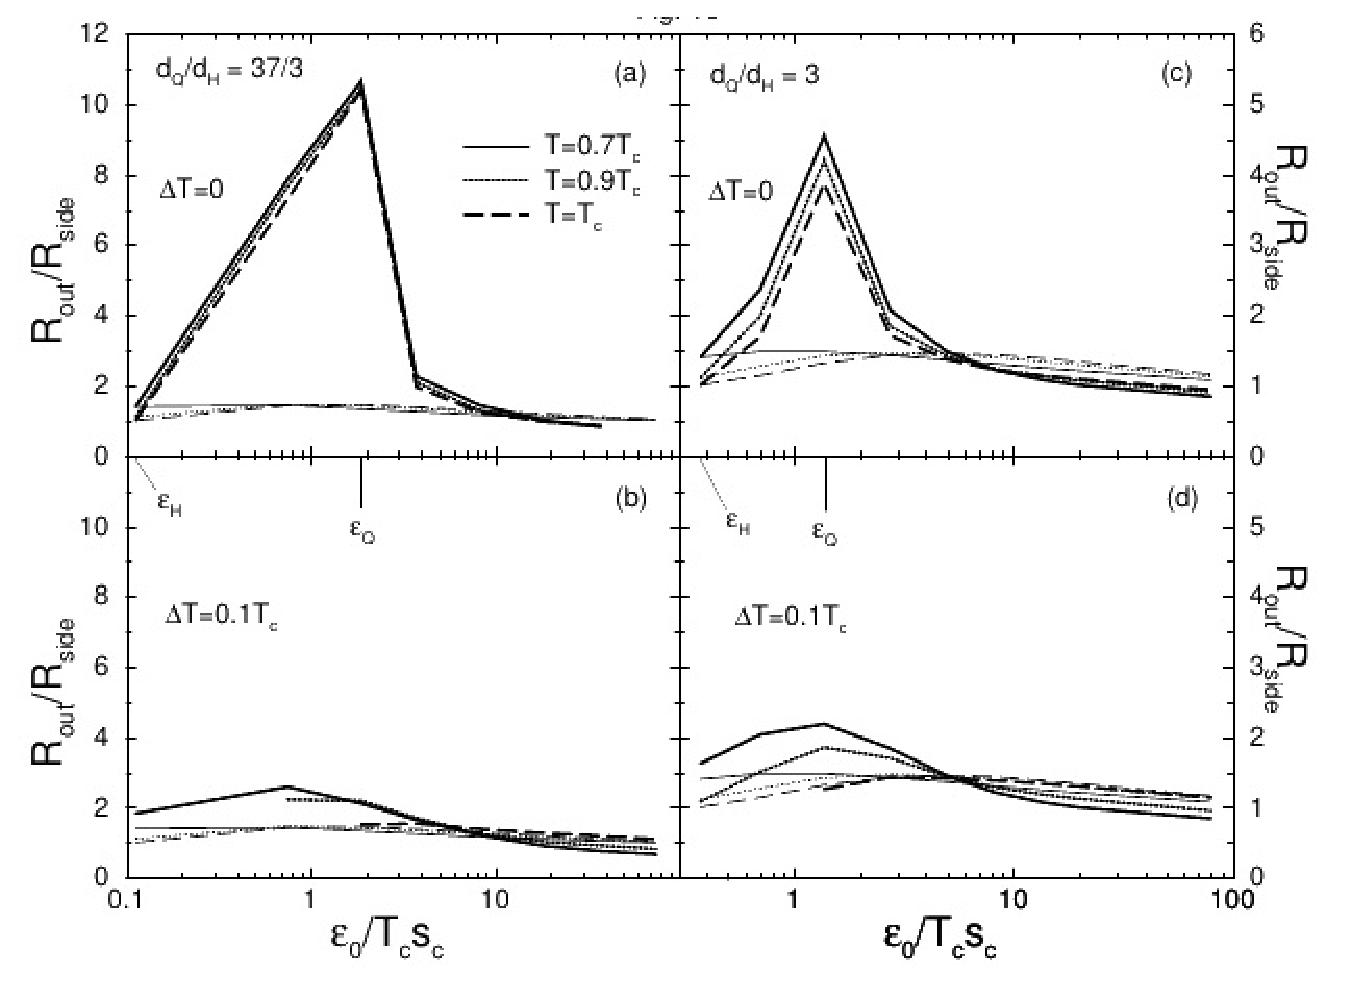
\includegraphics[width=1.\linewidth]{1pt-emissionDuration.eps}
                   \end{figure}
          \end{block}
          
          
          \column{.315\textwidth}
          \begin{block}{\bf \centering {\tiny Phys.Rev. C92 (2015) 1, 014904}}
            \begin{figure}[H]
              \includegraphics[width=1.\linewidth]{RiRootS.eps}
            \end{figure}
          \end{block}

          \column{.17\textwidth}
          \begin{block}{\bf \centering {\scriptsize {\color{ForestGreen} Observed:}}}
            {\scriptsize r-t correlations in expanding source reduce $R_{out}$ $\rightarrow$ $R_{out} / R_{side}$}
          \end{block}
          \vskip -0.4cm
          \begin{block}{}
            {\scriptsize Study of femtoscopy observables allows one {\color{red} to perform tune of the models to describe correctly collision dynamics}}
          \end{block}
        \end{columns}
        \note{According to earlier considerations it was predicted that ratio of $R_{out} / R_{side}$ should be 
          much greater than 1. Existing experimental data demonstrated a fact that the ratio is not so large and is very closed to unity. Firstly, it was considered as a puzzle, so called RHIC puzzle. In order to solve the problem, a tune
        of existing hydrodynamic models was performed to make shorter emission duration.}
      \end{frame}

      \begin{frame}
        \bf
        \frametitle{\bf \centering Femtoscopy with vHLLE+UrQMD}
        \vskip -.3cm
        \begin{block}{\bf \centering Iu. Karpenko, P. Huovinen, H.Petersen, M. Bleicher, Phys.Rev. C 91, 064901 (2015)}
          \begin{figure}[H]
            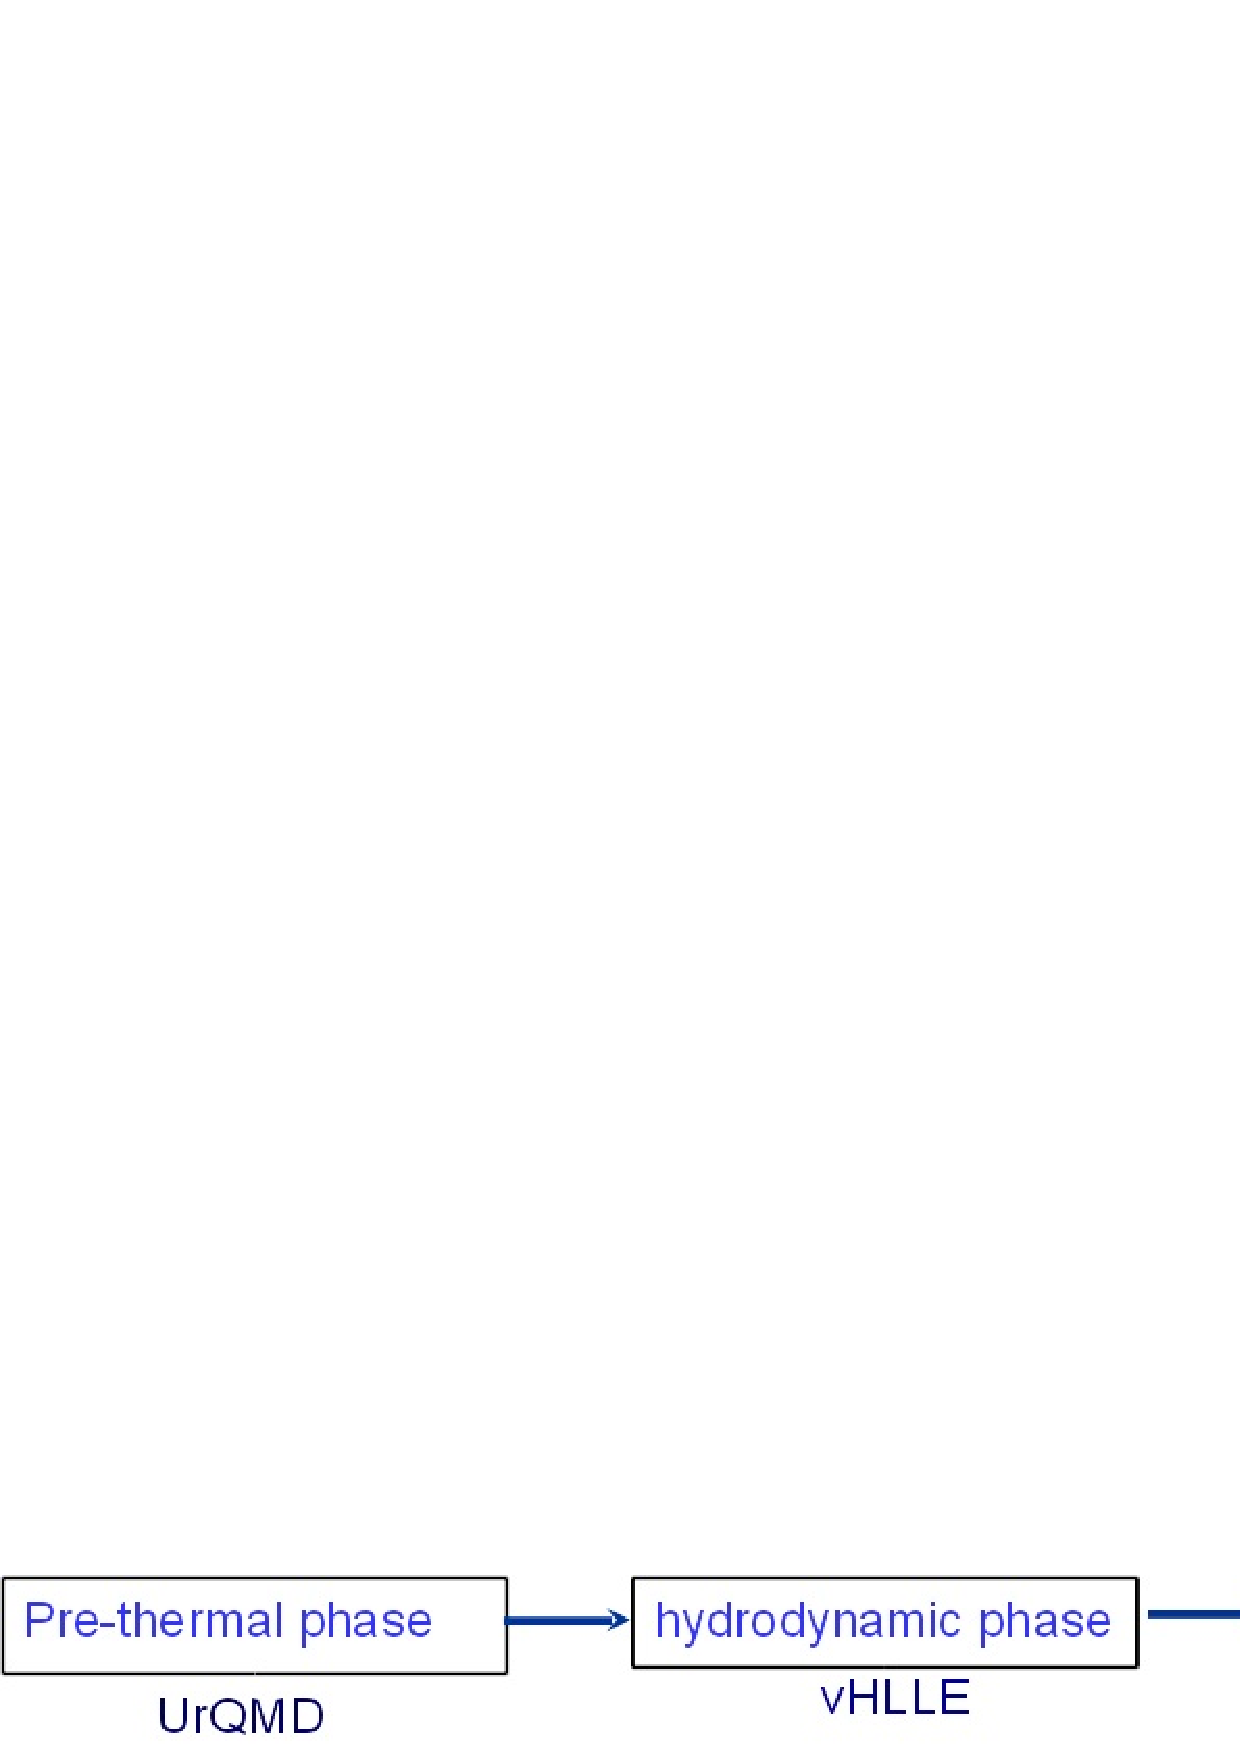
\includegraphics[width=1.\linewidth]{vHLLE_UrQMD_sandwich.png}
          \end{figure}
        \end{block}
        \vskip -.8cm
        \begin{columns}[t]    
          \column{.30\textwidth}
          \begin{block}{\bf \centering {\tiny Parameters $\tau_0$, $R_\perp$, $R_\eta$ and $\eta/s$ adjusted using basic
                observables in the RHIC BES-I region.}}        
            %\vskip -.3cm
            \resizebox{\columnwidth}{!}{%       
              \begin{tabular}{|l|l|l|l|l|}
                \hline
                $\sqrt{s_{\rm NN}}$~[GeV] & $\tau_0$~[fm/c] & $R_\perp$~[fm] & $R_\eta$~[fm] & $\eta/s$ \\ \hline
                7.7          &      3.2        &     1.4        &     0.5    &    0.2   \\ \hline
                8.8 (SPS)    &      2.83       &     1.4        &     0.5    &    0.2   \\ \hline
                11.5         &      2.1        &     1.4        &     0.5    &    0.2   \\ \hline
                17.3 (SPS)   &      1.42       &     1.4        &     0.5    &    0.15  \\ \hline
                19.6         &      1.22       &     1.4        &     0.5    &    0.15  \\ \hline
                27           &      1.0        &     1.2        &     0.5    &    0.12  \\ \hline
                39           &      0.9        &     1.0        &     0.7    &    0.08  \\ \hline
                62.4         &      0.7        &     1.0        &     0.7    &    0.08  \\ \hline
                200          &      0.4        &     1.0        &     1.0    &    0.08  \\ \hline
              \end{tabular}
            }
            \vskip 0.2cm
                   {\color{red} \scriptsize Model tuned by matching with existing experimental data from SPS and BES-I RHIC}
          \end{block}

          \column{.32\textwidth}
          \begin{block}{\bf \centering \scriptsize EoS to be used in the model}
            \begin{itemize}
            \item \tiny Chiral EoS - crossover transition \\ J. Steinheimer et al., J. Phys. G 38, 035001 (2011)
            \item \tiny Hadron Gas + Bag Model 1-st order phase transition \\ P. F. Kolb et al., Phys.Rev. C 62, 054909 (2000)
            \end{itemize}
          %  \vskip -.15cm
          %  \begin{figure}[H]
          %    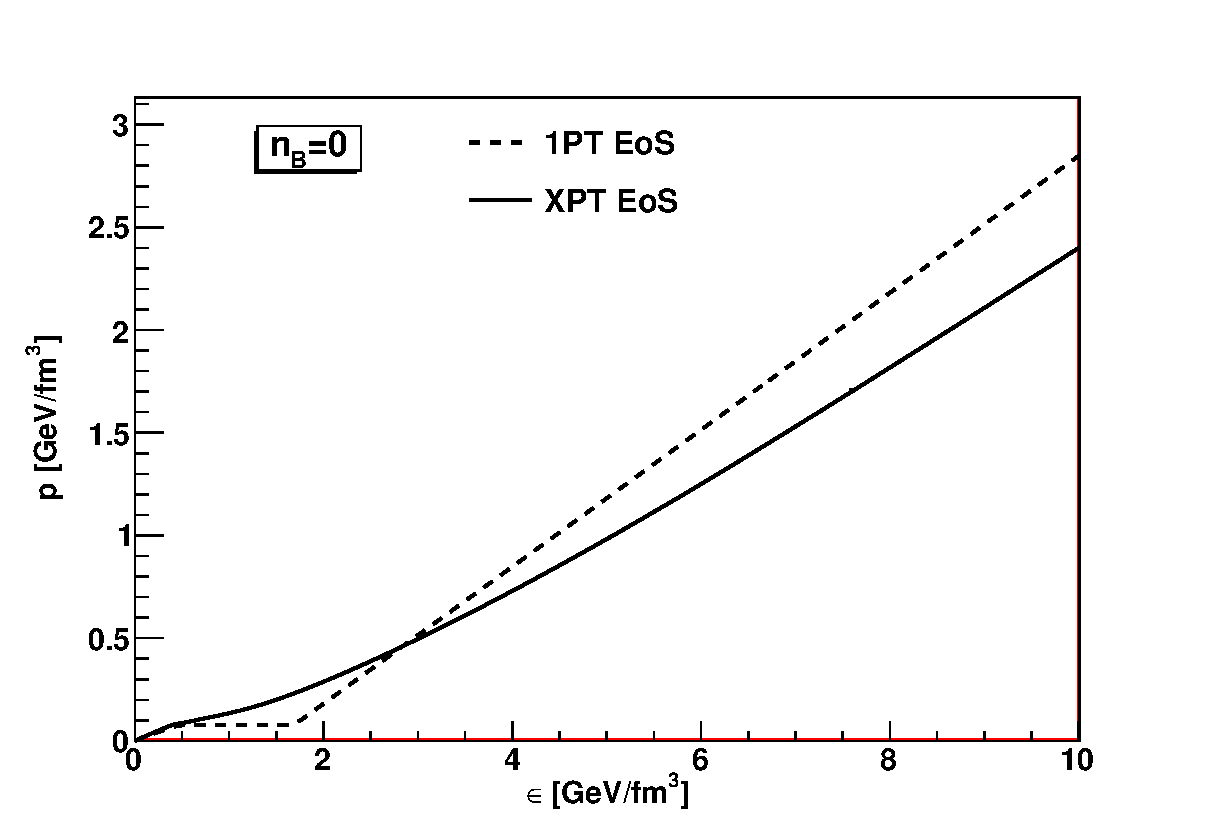
\includegraphics[width=1.01\linewidth]{eos.eps}
          %  \end{figure}
          \end{block}
          \vskip -0.4cm
          \begin{block}{}
            {\scriptsize {\color{blue} Hydrodynamic phase lasts longer with 1PT,
                especially at lower energies but cascade smears this difference.}}
          \end{block}

          \column{.32\textwidth}  
          \begin{block}{\bf \centering {\tiny Pion emission time}}
            \vskip -0.1cm
                   {\tiny
                     (a) - after hydrodynamic phase \\
                     (b) - after cascade
                   }
                   \vskip -0.45cm
                   \begin{figure}[H]
                     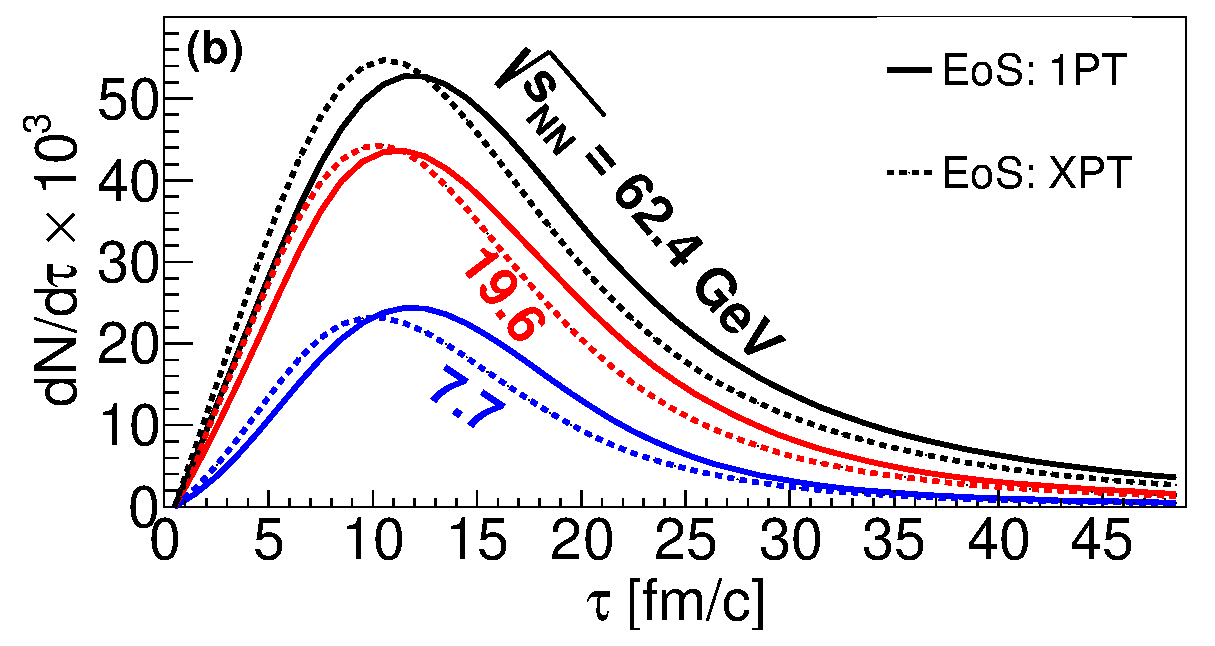
\includegraphics[width=1.\linewidth]{fig1a.eps} \\
                     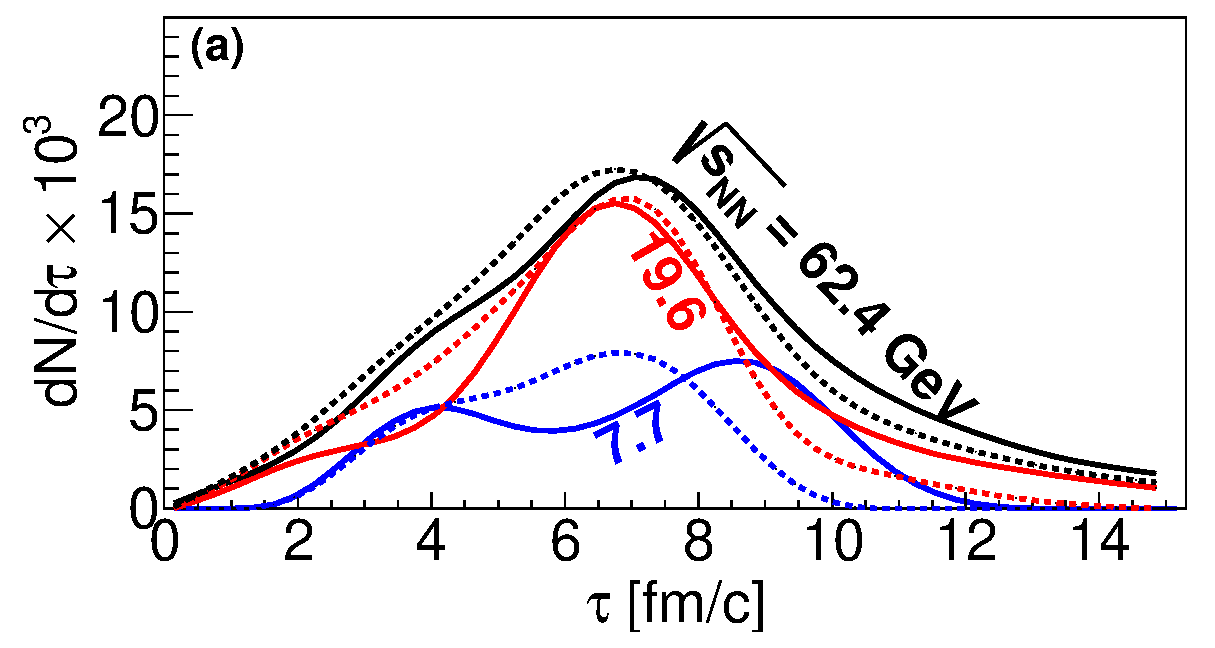
\includegraphics[width=1.\linewidth]{fig1b.eps}
                   \end{figure}
                   %\vskip -.7cm
          \end{block}
        \end{columns}
        \vskip -.3cm
        \begin{columns}[t]
          \column{.42\textwidth}
          %\begin{block}{\bf \centering {\tiny Ratios of 1D-projections of 3D correlation functions for two EoS}}
          %  \vskip -.2cm
          %  \begin{figure}[H]
          %    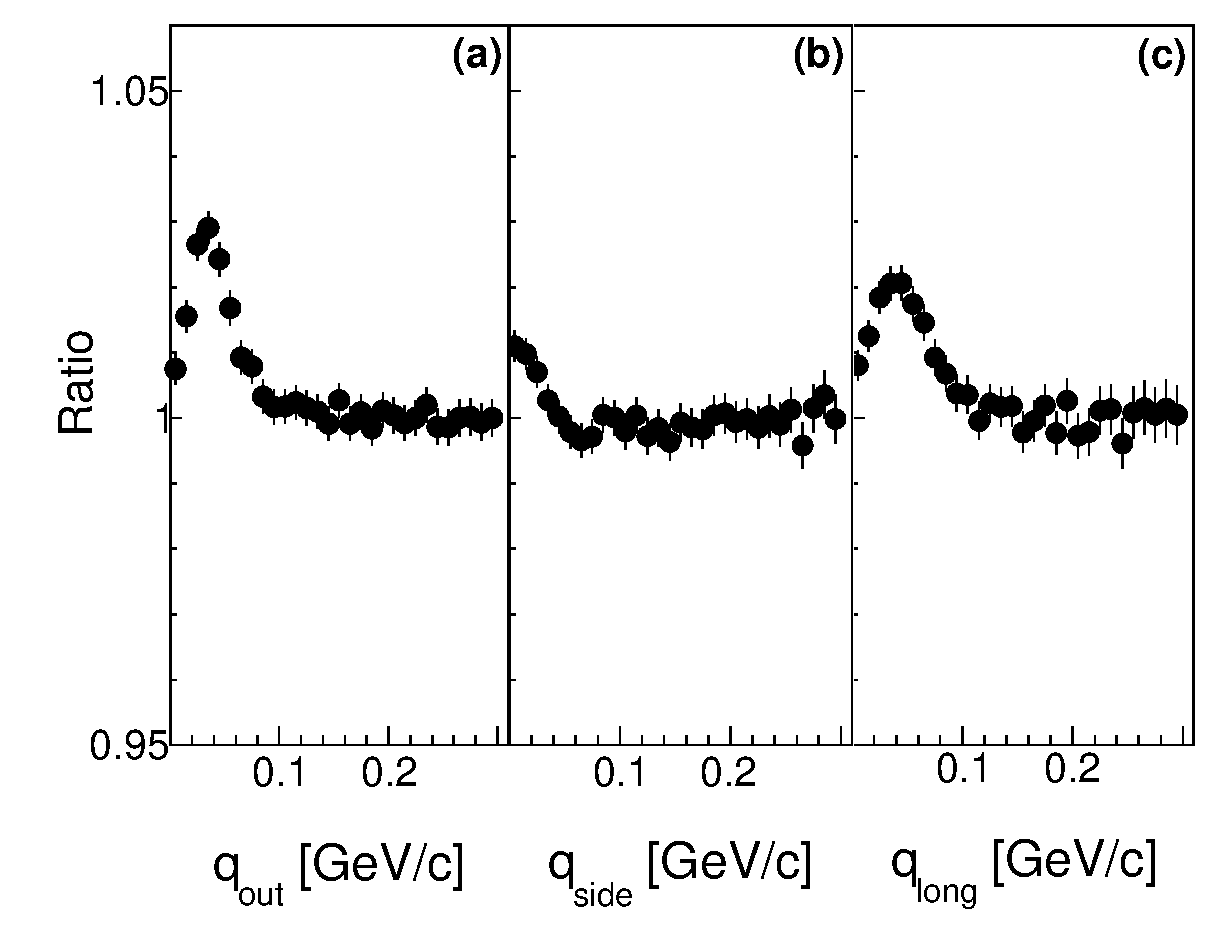
\includegraphics[width=1.0\linewidth]{fig3.eps}
          %  \end{figure}
          %\end{block}
          \column{.49\textwidth}
          %       {\footnotesize
          %         \begin{block}{\bf \centering Analysis:}
          %           \begin{center}
          %            AuAu @ $\sqrt{s_{NN}} = 7.7$ GeV \\
          %            Centrality 0-5\% \\
          %            $k_{T} = (0.15-0.25)$ GeV/c
          %          \end{center}
          %        \end{block}
          %        \vskip -.3cm
          %        \begin{block}{}
          %          \begin{itemize}
          %          \item Difference is seen in the ``out'' and ``long''
          %            directions.
          %          \item Ratios in the ``out'' and ``long'' directions reach values up to 1.03 at small
          %            $q_{out}$ and $q_{long}$.
          %          \end{itemize}
          %        \end{block}
          %      }
        \end{columns}
        \note{
          \vskip -0.6cm
          \scriptsize As a candidate for our studies the vHLLE+UrQMD model has been chosen. It is a model of ``sandwich''-like type
          consisting of three stages to be used sequentially for describing collision evolution. Initial stage of collision and hadronic cascade are realized via UrQMD model,
          meanwhile hydrodynamic stage includes calculations done by the author of the model. To get more detail on it, one is reffered to the publication. The model allows one to
          perform calculations assuming two different scenarios of nuclear matter EoS to be used, croosover and a first order phase transition. Basic parameters of the model
          have been tuned using experimental data from SPS and the BES program. The tuning aimed to describe reasonably well basic particle spectra, but did not cover femtoscopic
          observables. So, femtoscopy observables derived from the model are free ones and not restricted by any "femtoscopy" adjustments.
          The main reason that convinced us to use the model for our studies is a visible difference in emission of particles, depending on the EoS used, as after hydrodynamic phase
          well as hadronic cascade. The energy is lower the difference is bigger one can observed after the hydrodynamic stage. Despite the hadronic cascade smears the difference,
          it still remains visible, thus it could lead to different behaviour of femtoscopic observables depending on EoS.}
      \end{frame}

      \begin{frame}
        \bf
        \frametitle{\bf \centering 3D Pion radii versus $m_{T}$ with vHLLE+UrQMD }
        \begin{columns}[c]
          \column{.36\textwidth}
          \vskip -.3cm
          
          % \vskip -.75cm
          \begin{block}{{\bf \scriptsize  Phys. Rev. C 96, 024911 (2017)}}
            \begin{figure}[H]
              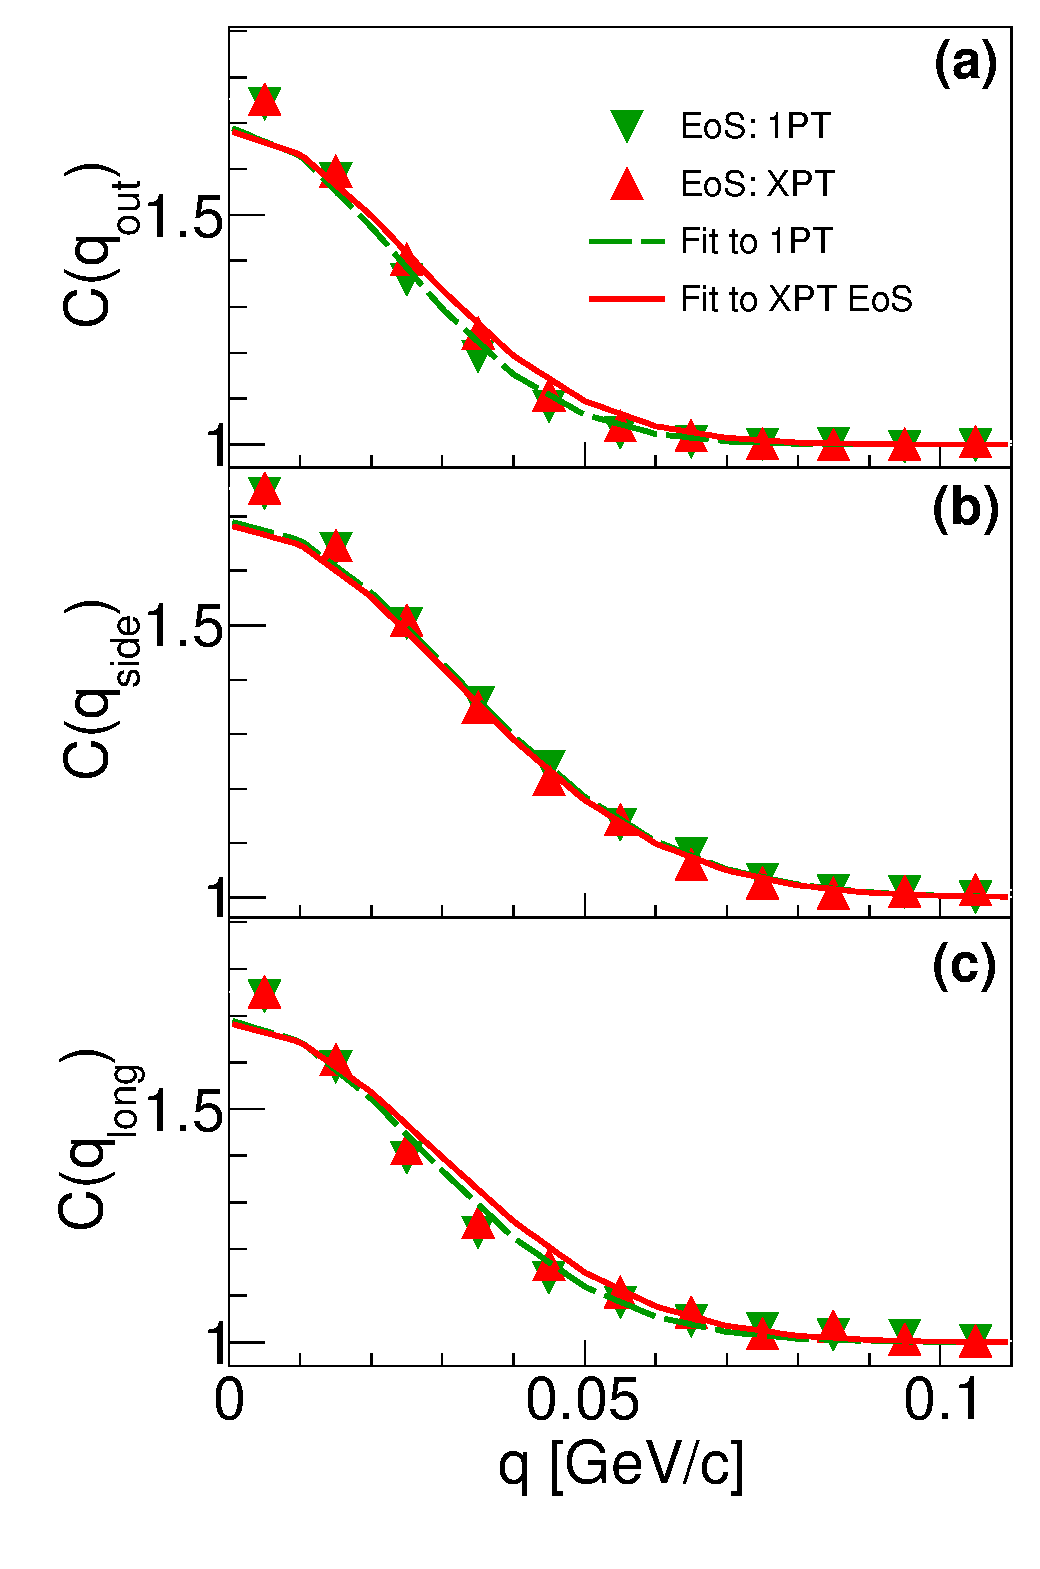
\includegraphics[width=1.\linewidth]{fig2.eps}
            \end{figure}
          \end{block}
          \column{.63\textwidth}
          \vskip -.3cm
          \begin{block}{\bf \centering {\tiny Comparison of extracted radii with the STAR data}}
            % \vskip .3cm
            \begin{figure}[H]
              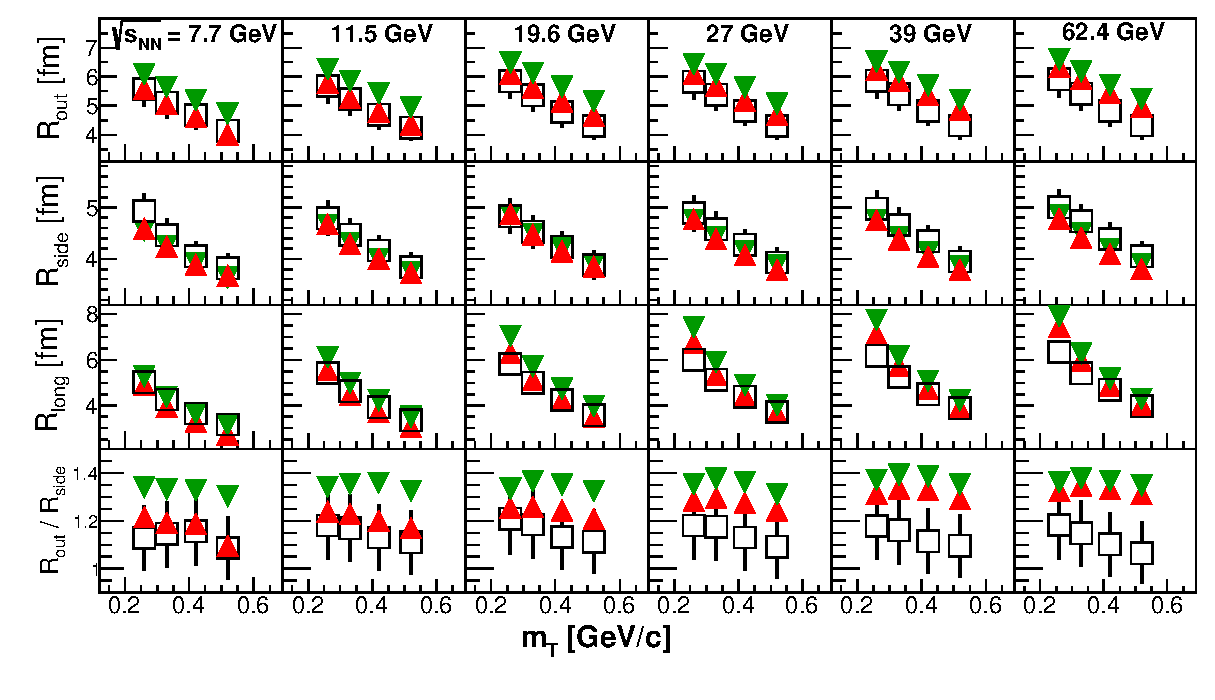
\includegraphics[width=1.0\linewidth]{fig4_poster.eps}
            \end{figure}
          \end{block}
          % \begin{block}{}
          %   {\scriptsize
          %     \begin{itemize}
          %     \item {\color{Red} EoS with a crossover in the fluid phase} results in a quite reasonable reproduction of 3D pion femtoscopic radii measured by
          %       the STAR collaboration (empty squares).
          %     \item {\color{ForestGreen} EoS with a first-order phase transition} leads to fact that the ``out'' and ``long'' Gaussian femtoscopic radii are systematically larger
          %      if comparing with the {\color{Red} crossover EoS}; the ``side'' radii coincide for both types of EoS.
          %  \end{itemize}
          % }
          %\end{block}
          \vskip -.35cm
          \begin{block}{}
            {\color{red} Crossover EoS} ``works'' better for lowest collision energies.
          \end{block}
          \vskip -.35cm
          \begin{block}{}
            {\scriptsize
              \begin{itemize}
              \item $R_{out}$ (XPT) at high energies and $R_{out}$ (1PT) at all energies are slightly overestimated
                %$\rightarrow$
                %{\color{red} an indication to reduce the emission time in the model.}
              \item $R_{out, long}$ (1PT) > $R_{out, long}$ (XPT) by value of $\sim$ 1-2~fm. 
              \end{itemize}
            }
          \end{block}
        \end{columns}
        \note{
          Since we chose a model to be used for our studies, the first step
          we did, was to extract femtoscopic radii directly from the model
          to compare them with existing eperimental data. As a data base,
          we took the pion STAR data got from the RHIC BES program.
          Calculations with the crossover EoS are presented by red color,
          meanwhile those for the 1PT scenario - by green color. If
          comparing between both scenarios, one can see that the crossover
          scenario work better for the radii description, especially,
          when considering $R_{out} / R_{side}$ ratio at lowest energies
          available. 1PT-scenario overestimates the radii by value of about
          1fm for out and long direction. THhis fact could be considered as
          an indication to reduce the emission time in the model.
        }
      \end{frame}

      \begin{frame}
        \frametitle{\bf \centering $R_{out} / R_{side}$  with vHLLE + UrQMD model}
        \bf
        \vskip -1.3cm
        \begin{columns}[t]
          \column{.35\textwidth}
          \begin{block}{}     
            \begin{figure}[H]
              \includegraphics[width=1.0\linewidth]{RoutRside_STAR_ALICE.png}
            \end{figure}
          \end{block}

         % \column{.3\textwidth}
         
         % \vskip -0.25cm
          %\begin{block}{\bf \centering Model calculations:}
          %  \begin{itemize}
          %  \item \scriptsize Optimal description of the femtoscopic radii
          %  requires about 1~fm shorter duration of pion emission with the present setup of the model.       
          %  \end{itemize}
          %\end{block}
          
          \column{.48\textwidth}
                 {\scriptsize 
                   \begin{block}{\bf \centering \scriptsize Exp. data:}
                     $R_{out} / R_{side}$ and $R_{out}^{2} - R_{side}^{2}$ as a function of
                     $\sqrt{s_{NN}}$ at a fixed $m_{T}$ demonstrate a wide maximum near
                     $\sqrt{s_{NN}} \approx$ 20 GeV
                   \end{block}
                 }
                 \vskip -0.4cm
           \begin{block}{\bf \centering \scriptsize Our calculations: }
             \begin{figure}[H]
               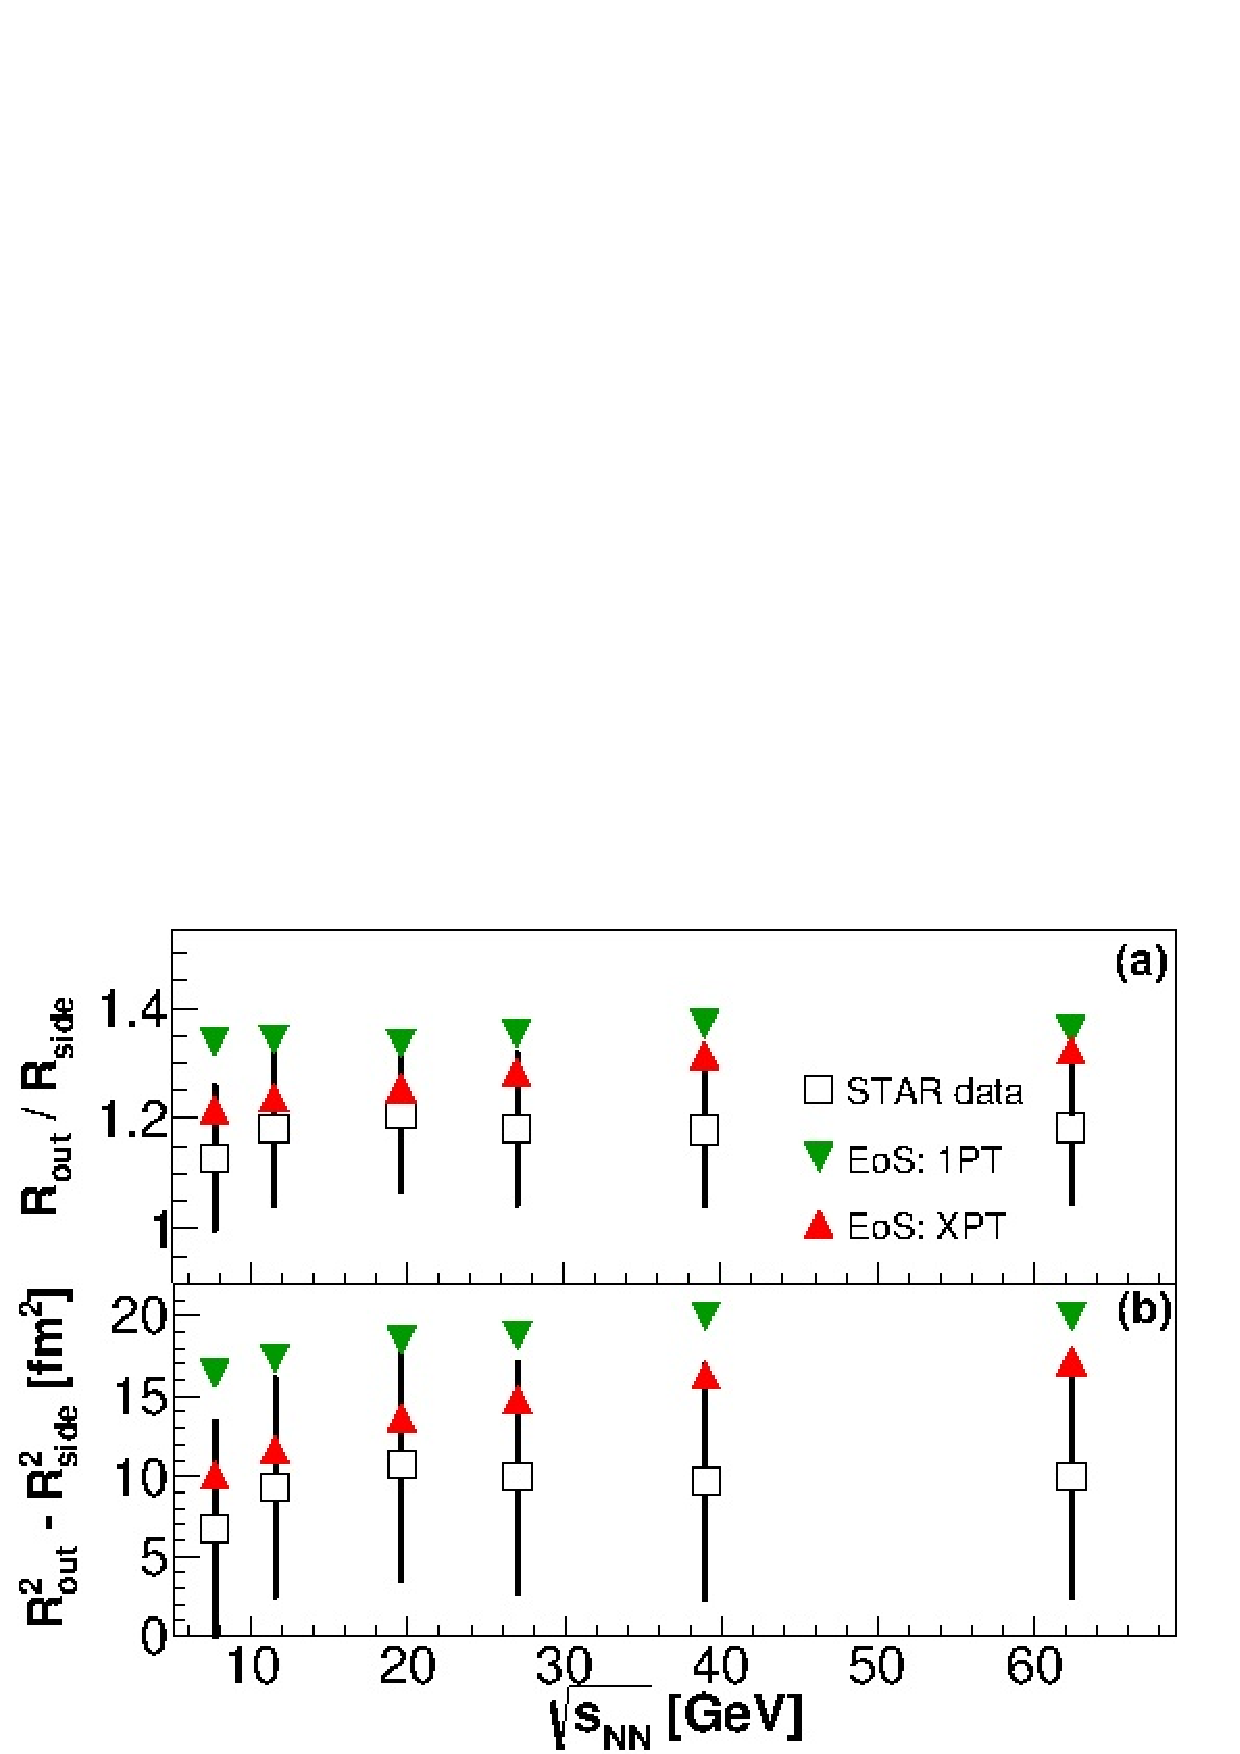
\includegraphics[width=1.0\linewidth]{fig5_modif.pdf}
             \end{figure}
             \vskip -0.65cm
             {\scriptsize $R_{out} / R_{side}$ (XPT) agrees with almost all STAR data points within rather large systematic errors,
             while $R_{out} / R_{side}$ (1PT) overestimates the data.}
          \end{block}
        \end{columns}
        \vskip -1.cm
       % \begin{columns}[t]
        %  \column{.33\textwidth}
        %  \column{.64\textwidth}
         % \begin{block}{}
           % \begin{itemize}
         % \item
          %  {\color{red} Does a new set of parameters help us to accommodate the femtoscopic radii?}
          %  \end{itemize}
       %   \end{block}
       % \end{columns}
        \note{Another point we got from the model covers not only
          $R_{out} / R_{side}$ but difference of its squares. This part of
        analysis was motivated by the fact that the difference at a fixed
        $m_{T}$-value shows a wide maximum around 20 GeV of collision energy in
        c.m.s. as obtained from experimental data. Calculations we performed are
        agreed with the STAR data points with large systematic errors if assuming
        the crossover scenario in the model. 1PT-scenario overestimates as ratio
        as well as difference of considering radii.
        }
      \end{frame}

      
      \begin{frame}
        \bf
        \frametitle{Ratio of $R_{out, side, long}(1PT) / R_{out, side, long}(XPT)$ vs. $\sqrt{s_{NN}}$}
        \vskip -0.75cm
        \begin{columns}[t]
          \column{.38\textwidth}
          \begin{block}{}
             \begin{figure}[H]
               \includegraphics[width=1.0\linewidth]{Rout_diffEoS.png} \\
            % \end{figure}
            %  \begin{figure}[H]
               \includegraphics[width=1.0\linewidth]{Rside_diffEoS.png} \\
             % \end{figure}
             %  \begin{figure}[H]
               \includegraphics[width=1.0\linewidth]{Rlong_diffEoS.png}
             \end{figure}
          \end{block}
          \column{.49\textwidth}
          \begin{block}{}
            \begin{itemize}
            \item $R_{side}$ practically coincide for both scenarios
            \item $R_{out}$ and $R_{long}$  for 1PT EoS are greater than for XPT EoS 
              demonstrating a strong $k_{T}$-dependence
            \end{itemize}
          \end{block}
          \begin{block}{\bf \centering Why?}
            The difference comes from a {\color{red} weaker transverse flow developed in the fluid phase}
            with 1PT EoS as compared to XPT EoS  and its {\color{red} longer lifetime} in 1PT EoS
          \end{block}
        \end{columns}
        \note{
          In the slide ratios of corresponding radii for the 1PT and crossover
          scenarios are presented. Transverse momenta of pion pair are divided into
          four bins. $R_{side}$ has practically the same order of magnitude
          for both scenarios.
          $R_{out}$ and $R_{long}$ tend to be greater for the 1PT-scenario and
          demonstrate a clear $k_{T}$-dependence especially for lowest values of
          $k_{T}$. A weaker transverse flow in the fluid phase
          and its longer lifetime in the 1PT EoS if comparing with the crossover
          EoS could be considered as a possible explanation. 
        }
      \end{frame}
      
      \begin{frame}
        \bf
         \frametitle{\bf \centering \footnotesize Kaon correlation functions with vHLLE+UrQMD { \color{red} (NEW!)}}
         \vskip -.75cm
         \begin{columns}[t]
           \column{.50\textwidth}
           \begin{block}{\bf \centering Pions:}
             \begin{figure}[H]
               \includegraphics[width=1.0\linewidth]{proj3D_pions.png}
               \end{figure}
           \end{block}
            \vskip -.3cm
            \begin{block}{\bf \centering Kaons:}
             \begin{figure}[H]
                 \includegraphics[width=1.0\linewidth]{proj3D_kaons.png}
             \end{figure}
           \end{block}
           \column{.39\textwidth}
           \begin{block}{\bf \centering Analysis:}
             \begin{itemize}
             \item \footnotesize AuAu, $\sqrt{s_{NN}} = 11.5$ GeV
             \item \footnotesize $N_{events} \approx 400 000$
             \item \footnotesize Standard 3D Gaussian fit used
             \end{itemize}
           \end{block}
           \vskip -.2cm
           \begin{block}{}
             \begin{itemize}
             \item Projections of {\color{red} 3D-kaon correlation functions} on out-side-long directions are {\color{red} more Gaussian}
             \item {\color{red} XPT CF projections} on {\color{red} long direction} are {\color{red} visibly wider} than 1PT especially {\color{red} for kaons}
             \end{itemize}
           \end{block}
         \end{columns}
         \note{
          As a continuation of our model studies and addition to the pion results,
          we have done a preliminary analysis for charged kaons. Details of the
          analysis are presented in the slide. The analysis revealed two remarkable
          facts. The first one states a more gaussian form of all projections
          of 3D correlation function for kaons. Also, in case of kaons long
          projection of correlation function is wider for the 1PT-scenario in the
          model.
        }
       \end{frame}

      \begin{frame}
        \frametitle{\bf \centering Pion \& Kaon radii vs. $m_{T}$ with vHLLE+UrQMD}
        \begin{figure}[H]
            \includegraphics[width=.68\linewidth]{AuAu_077.pdf}
        \end{figure}
      \end{frame}

       \begin{frame}
        \frametitle{\bf \centering Pion \& Kaon radii vs. $m_{T}$ with vHLLE+UrQMD}
        \begin{figure}[H]
          \includegraphics[width=.68\linewidth]{AuAu_115.pdf}
        \end{figure}
       \end{frame}
      

       \if 0
      \begin{frame}
        \bf
        \frametitle{\bf \centering Pions \& Kaon radii vs. $m_{T}$ with vHLLE+UrQMD}
        \vskip -0.5cm
        \begin{columns}[t]
          \column{.49\textwidth}
          \begin{figure}[H]
            \includegraphics[width=1.0\linewidth]{AuAu_077.pdf}
          \end{figure}
          \column{.49\textwidth}
           \begin{figure}[H]
            \includegraphics[width=1.0\linewidth]{AuAu_115.pdf}
          \end{figure}
        \end{columns}
        \begin{block}{}
          \begin{itemize}
          \item Pion and kaon radii are mainly larger for the 1PT-scenario
          \item Approximate $m_{T}$-scaling for pions and kaons only for $R_{side}$
            is observed
          \end{itemize}
        \end{block}
        \note{
          $m_{T}$-dependences of extracted radii for two lowest energies of BES and,
          simulataneously, in the NICA energy range are shown. As in the case of
          pions we have already considered, the kaon radii extracted from
          the calculations with the 1PT-scenario are mainly larger with those got
          from the crossover ones. The distributions demonstrate an approximate
          $m_{T}$-scaling for both types of particles in case of $R_{side}$.
        }
      \end{frame}
      \fi

      \begin{frame}
        \bf
        \frametitle{\bf \centering Summarising ...}
        \begin{itemize}
        \item Hydro phase lasts longer with 1PT.  
        \item vHLLE+UrQMD with XPT-scenario describes BES-I STAR femtoscopy radii at $\sqrt{s_{NN}}$ = 7.7, 11.5 GeV  better than the 1PT-scenario. 
        \item $R_{long}$ for 1PT is greater than for XPT.%,  difference is rather small for low energies. 
        \item $R_{out} / R_{side}$ for 1PT also is greater than for XPT.%, difference is rather small for low energies.
        \item First results with kaon femtoscopy look promising and this study is planned to be continued.
        \end{itemize}
      \end{frame}

      \begin{frame}
        \bf
        \frametitle{\bf \centering Package for Femtoscopic Analysis}
        \vskip -0.8cm
        \begin{columns}[t]
          \column{.49\textwidth}
          \begin{block}{\bf \centering {\footnotesize {\color{red} Femtoscopy}}}
            \begin{itemize}
            \item \scriptsize Inherited from STAR (StHbtMaker) and ALICE (AliFemto)
            \item \scriptsize Keeps the same hierarchy as in ALICE (PckgName/, PckgNameUser/, macros/)
            \item \scriptsize Works with ROOT 5 and 6
            \item  \scriptsize Lighter than ancestors:
              \begin{itemize}
              \item \scriptsize Most of STAR-developed classes replaced with ROOT ones
              \item \scriptsize Better compression, smaller sizes
              \end{itemize}
            \item \scriptsize Implemented running options (INDEPENDENT on experiment-dependent software):
              \begin{itemize}
              \item \scriptsize Standalone mode – compile with g++ (clang) and run on your “laptop”
              \item \scriptsize Maker; Tasks will be also implemented
              \end{itemize}
            \end{itemize}
          \end{block}

          \column{.49\textwidth}
          \begin{block}{\bf \centering {\footnotesize {\color{ForestGreen} Data formats (DST)}}}
            \begin{itemize}
            \item  \footnotesize General-purpose data format for Monte Carlo generators - McDst~\url{https://github.com/nigmatkulov/McDst}
            \item  \footnotesize Similar to UniGen (developed at GSI)
            \item  \footnotesize Lighter, faster, easy expandable, works with ROOT 5 and 6, g++ (clang)
            \item  \footnotesize Possibility to add converters from other generators: Terminator, EPOS, AMPT ...
            \item  \footnotesize Group has a positive experience on the data format developments:
              \begin{itemize}
              \item  \footnotesize PicoDst format in STAR (standard data format for physics analysis)
              \end{itemize}
            \end{itemize}
          \end{block}
        \end{columns}
      \end{frame}

      \begin{frame}[fragile]
        \bf
        \frametitle{\bf \centering Package for Femtoscopic Analysis}
        \vskip -.83cm
        \begin{columns}[t]
          \column{.58\textwidth}
          \begin{block}{\bf \centering \scriptsize Output ROOT tree:}
            \begin{figure}[H]
              \includegraphics[width=1.\linewidth]{FemtoPack_example.png}
            \end{figure}
          \end{block}
          \vskip -0.3cm
          \begin{block}{\bf \centering \scriptsize It allows:}
            \begin{itemize}
            \item \scriptsize To set track cuts, particle pair cuts, number of events to be used for mixing ...
            \item \scriptsize To get 1D and 3D correlation functions for a set of $k_{T}$-bins
            \item \scriptsize To switch on / off different physics effects (QS, FSI ...)
            \end{itemize}
          \end{block}

          \column{.41\textwidth}
          \begin{block}{\bf \centering \tiny Main macro to define conditions of user's analysis}
            \vskip -0.33cm
                   {\tiny
                     \begin{lstlisting}[language=C++,basicstyle=\tiny\ttfamily,keywordstyle=\color{red}]
int main(int argc, char* argv[]) {
...
 // Create and set track cut
trackCut->setPdgId(particlePdg);
trackCut->setEta(-1., 1.);
trackCut->setPt(0.15, 1.55);
trackCut->setMass(particleMass);
...
// Set how many events to mix
hbtAnalysis->setNumEventsToMix(10);
...
// Lednicky weight generator
hbtWeight->setPairType(pairType);
hbtWeight->setCoulOn();
hbtWeight->setQuantumOn();
hbtWeight->setStrongOff();
hbtWeight->set3BodyOff();
...
// Create 1D correlation function
// integrated over kT
StHbtModelQinvCorrFctn *oneDim =
new StHbtModelQinvCorrFctn
("hTheorQinv", 40, 0., 0.4);
// Create 3D correlation function
// integrated with kT binning
StHbtModelBPLCMS3DCorrFctnKt *threeDim =
new StHbtModelBPLCMS3DCorrFctnKt
("hTheorBPLCMS", 80, -0.4, 0.4, 4,
0.15, 0.59);
}
\end{lstlisting}
}
\end{block}
\end{columns}     
\end{frame}

      \begin{frame}
        \frametitle{\bf \centering {\color{red} Where will it be studied?}}
        \bf
        \vskip -0.25cm
        \begin{columns}[t]
          \column{.49\textwidth}
          \vskip -0.5cm
          \begin{block}{\bf \centering MPD Layout:}
            \begin{figure}[H]
              \includegraphics[width=1.\textwidth]{mpd.png} 
            \end{figure}
          \end{block}
          \vskip -0.3cm
                 {\tiny 
                   \begin{block}{\bf \centering Participants:}
                     
                     \begin{columns}[t]
                       
                       \column{.49\textwidth}
                       \vskip -0.4cm
                       % \vspace -1cm
                       \begin{itemize}
                         %\item JINR, Dubna
                       \item Tsinghua University, Beijing, China
                       \item GSI, Darmstadt, Germany
                       \item WUT, Warsaw, Poland
                       \end{itemize}
                       
                       \column{.49\textwidth}
                       \vskip -0.3cm
                       \begin{itemize}
                       \item MEPhI, Moscow, Russia 
                       \item INR, RAS, Russia
                       \item PPC BSU, Minsk, Belarus
                       \item Dubna, JINR, Russia
                       \end{itemize}           
                     \end{columns}
                   \end{block}
                 }
                 
                 \column{.49\textwidth}
                        {\tiny
                          \vskip -0.5cm
                          \begin{block}{\bf \centering Benefits:}
                            %               \begin{columns}[t]
                            %                 \column{.23\textwidth}
                            \begin{itemize}
                            \item Hermeticity, $2\pi$-acceptance in azimuth
                            \item 3D-tracking (TPC, ECT)
                            \item Vertex high-resolution (IT)
                              %                \end{itemize}
                              %                \column{.43\textwidth}
                              %                \begin{itemize}
                            \item Powerful PID (TPC, TOF, ECAL)
                              \begin{itemize}
                              \item  {\tiny$\pi, K$ up to 1.5 GeV/c}
                              \item {\tiny$K, p$ up to 3 GeV/c}
                              \item {\tiny$\gamma, e$ from 0.1 GeV/c up to 3 GeV/c}
                              \end{itemize}
                              %                 \end{itemize}
                              %                 \column{.23\textwidth}
                              %                 \begin{itemize}
                            \item Precise event characterization (FHCAL)
                            \item Fast timing and triggering (FFD)
                            \item Low material budget
                            \item High event rate (up to 7 kHz) 
                            \end{itemize}
                            %              \end{columns}
                          \end{block}
                        }
                        \vskip -0.3cm
                        \begin{block}{\bf \centering Realization progress:}
                          %\vskip 0.40cm
                          %  \begin{center}
                          {\scriptsize
                            \begin{itemize}
                              % {\tiny \item TDR - completed / close to  completion }
                            \item Preparation for / start of mass production
                            \item First stage is planned to be started in {\color{red} 2021} 
                            \item Second stage and full commissioning (IT + end-cups) - {\color{red} 2023}
                            \end{itemize}
                          }
                          %  \end{center}
                          
                        \end{block}
        \end{columns}      
      \end{frame}

      \begin{frame}
        \bf
        \frametitle{\bf \centering \scriptsize Femtoscopy \& correlations activities within RFBR mega grant}
        \vskip -.25cm
        \begin{block}{}
          Activity has been supported by the RFBR grant for a period of three years (2019-2021) \\
            {\color{red} Aim:} {\scriptsize Study of collective effects and dynamics of quark-hadron phase transitions via femtoscopic correlations of
            hadrons and factorial moments of particle multiplicity at the NICA energies}
        \end{block}
        \vskip -.75cm
        \begin{columns}[t]
          \column{.49\textwidth}
          \begin{block}{\bf \centering Our physics to be studied:}
            \begin{itemize}
            \item \scriptsize {\color{red} Development} of data analysis methods and software to be integrated in the
              {\color{red} MPD software environment}
            \item \scriptsize {\color{red} Analysis} of simulated events with different event generators (in particular, UrQMD+vHLLE) at the
              {\color{red} NICA energies}
            \item \scriptsize {\color{red} Understanding} dependence of femtoscopic radii and scaled factorial moments of particle multiplicity
              on the initial conditions and properties of nuclear matter EoS
            \end{itemize}
          \end{block}
          \column{.49\textwidth}
          \begin{block}{\bf \centering Our the most future plans:}
            \begin{itemize}
            \item \scriptsize {\color{blue} Software development} for femtoscopic analyses \& factorial moments of multiplicity distributions
            \item \scriptsize {\color{blue} Femtoscopic analysis} for pions and kaons (correlation functions, source functions ...)
              for the events simulated (model investigations)
            \item \scriptsize {\color{blue} Study of detector effects} on femtoscopic measurements to be taken into account when doing analysis for
              reco-output from MPD 
            \end{itemize}
          \end{block}
        \end{columns}     
      \end{frame}

      \begin{frame}
        \bf 
        \frametitle{}
        \begin{figure}[H]
          \includegraphics[width=1.\textwidth]{wpcf2019.png} 
        \end{figure}
        \begin{center}
        {\Huge  Thank you for your attention!}
        \end{center}
      \end{frame}      
      \end{document}
